\section{Einleitung}

\begin{frame}
  \begin{itemize}
  \item Ziel: Leitfähigkeiten der Ionenkanäle ermitteln
  \item Basis Bachelorarbeit von Anne Kloskowki
  \item Erreicht:
    \begin{itemize}
    \item alternative Variatoren, Selektoren und Replacer
    \item GUI
    \item schnellerer Code ($>3\times$ speedup); Nebenläufigkeit von Konfigurationen
    \item persistente Ausgabe (Datei, Zeitstempel)
    \end{itemize}
  \end{itemize}
\end{frame}


\subsection{Neuronenmodelle}

\begin{frame}
  \begin{itemize}
  \item 4 Neuronenklassen
    \begin{itemize}
    \item regular spiking
    \item fast spiking
    \item intrinsic bursting
    \item chattering
    \end{itemize}
  \end{itemize}
\end{frame}




\section{Genetischer Algorithmus}

\subsection{Einleitung}

\begin{frame}
  \frametitle{Genetischer Algorithmus}
  \begin{columns}[T]
    \begin{column}{0.35\textwidth}
      \begin{itemize}
      \item 
      \item Schlussfolgerung
      \end{itemize}
    \end{column}
    \begin{column}{0.65\textwidth}
        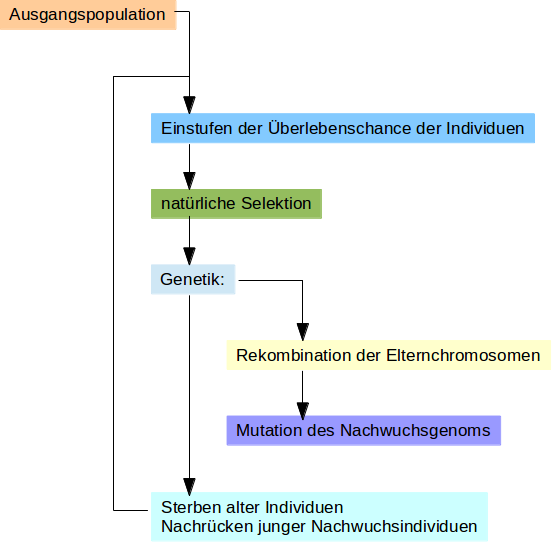
\includegraphics[width=\textwidth]{GenAlg-Diagramm.png}
        \captionsource{\tiny Evolutionäre Algorithmen zur Parametereinstellung
          in elektrophysiologischen Neuronenmodellen, Anne Kloskowski, 2013}
    \end{column}
  \end{columns}
\end{frame}

\subsection{Auswertung}

\begin{frames}
  \frametitle{Auswertung}
  
\end{frames}
  
